% Chapter 5

\chapter{Tests and Results} % Main chapter title

\label{Chapter5} % For referencing the chapter elsewhere, use \ref{Chapter5} 

\lhead{Chapter 5. \emph{Tests and Results}} % This is for the header on each page - perhaps a shortened title
This chapter presents the tests that we have taken to evaluate OptiX's characteristics from different points of view. Test results will be analysed in order to conclude OptiX's potential for Monte Carlo simulations. 

Note that all tests and implementations presented in this report is based on a working environment with:
\begin{itemize}
  \item \textbf{CPU:} Xeon E5504 (4M Cache, 2.00 GHz)
  \item \textbf{GPU:} Quadro 5000 (Compute Capability: 2.0, 352 CUDA cores, 120 GB/s)
  \item \textbf{OS:} 64-bit Debian Wheezy 
  \item \textbf{APIs:} OptiX 3.5 and CUDA 5.5. 
\end{itemize}
%----------------------------------------------------------------------------------------

\section{Effectiveness of Fast-Math}
Fast-math functions are built in CUDA architecture by using the "special function unit" in each multiprocessor, taking one instruction, whereas the CPU implementations can take dozens of instructions. The \textit{CUDA Programming Guide} does not list the speed difference, but according to the slides from Hwu's presentation \citep{hwu2009programming}, fast-math operations take 16 to 32 cycles per warp while standard operations are done in hundreds of cycles. Of course, here we are talking about the expensive functions (exp, sin, sqrt etc.), not simple multiplications or additions - those take about 20 cycles per warp. 

Fast-math functions get this speed improvement at the price of sacrificing their accuracy privilege. Note that few functions in CUDA follow the IEEE 754 specification \citep{cudaguide} and they only produce valid results for a given range of input values. The programming guide lists their maximum ULP (Unit in the Last Place) error information in \href{http://docs.nvidia.com/cuda/cuda-c-programming-guide/index.html#mathematical-functions-appendix}{Appendix D}. 
 
Developers can use the \textit{-use-fast-math} flag to force usage of intrinsics for the fast-math functions without changing source codes, so this would quickly give an idea of potential performance effect on the code.
\begin{figure}
\centering
\subfigure[Fast-math case]{
\label{Fig.sub.1}
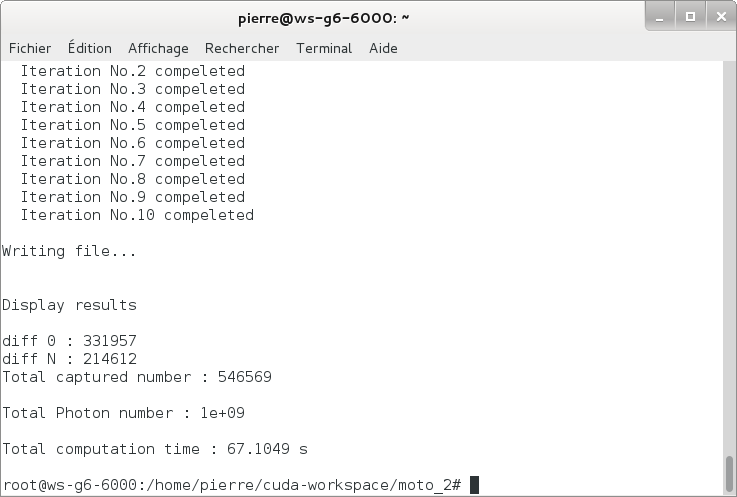
\includegraphics[width=0.7\textwidth]{Figures/fast.png}}
\subfigure[Normal case]{
\label{Fig.sub.2}
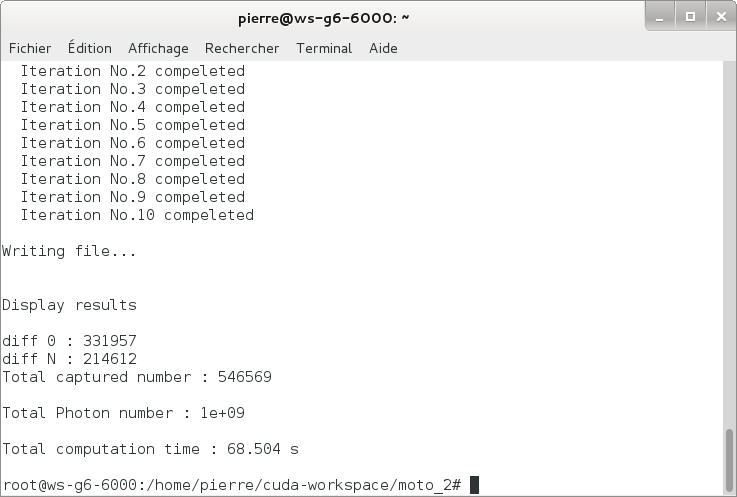
\includegraphics[width=0.7\textwidth]{Figures/standard.png}}
\caption{Comparison of fast-math functions and standard functions}
\label{fig:compa}
\end{figure}

\fref{fig:compa} shows test results on this effect. We find that fast-math has a slight speedup compared to normal operations. It indicates that among the entire calculation in OptiX kernel, arithmetic functions occupy a little part and therefore this acceleration is too hard to distinguish. Furthermore, since MODERATO doesn't require a high-standard accuracy, the amount of photons arrived on the detector is exactly the same in these two tests. In conclusion, fast-math functions doesn't effect our implementation's outputs. They can satisfy our arithmetic precision requirements and accelerate calculation performance. Note that the current implementation doesn't include many computationally intensive operations, the acceleration of fast-math will be more evident for a more complicated test. Likewise, fast-math might be not accurate enough for other serious simulations.
%----------------------------------------------------------------------------------------

\section{Degradation with Atomic Operations}
Atomic operations serialize the execution of parallel programs and therefore pull down computing performance. Some algorithms can be optimized to avoid this serialization, others may not. We did a test to know how serious the atomic will effect our implementation's performance (\fref{fig:ato}).
\begin{figure}
\centering
\subfigure[No counters]{
\label{Fig.sub1}
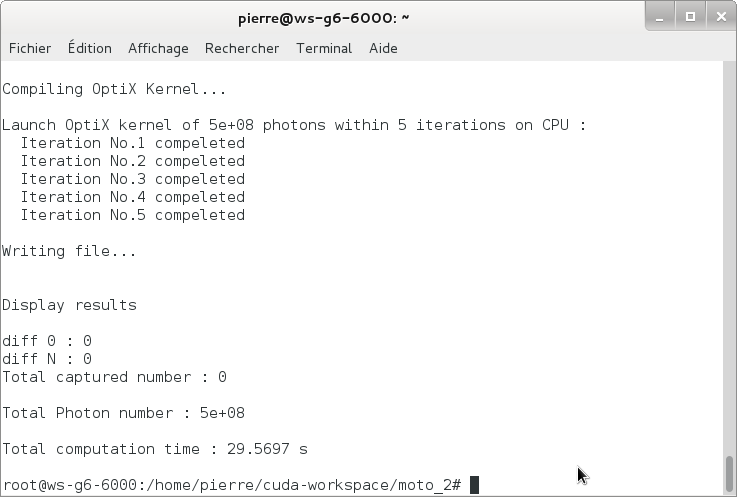
\includegraphics[width=0.7\textwidth]{Figures/noatomic.png}}
\subfigure[Atomic counters]{
\label{Fig.sub2}
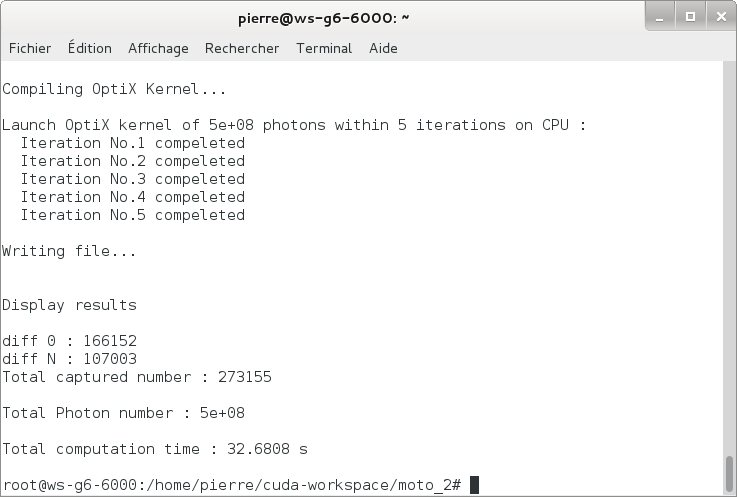
\includegraphics[width=0.7\textwidth]{Figures/atomic.png}}
\caption{Effectiveness of atomic operations}
\label{fig:ato}
\end{figure}

Fifteen counter variables require atomic addition. For the first test, we comment all these additions so the counter works no more. Then a second test deactivates the comment and gets a delay for about 3.1 seconds ($\approx 10\ \%$). This degradation is considerable because we haven't employed too many atomics. For further implementation, changing algorithms to avoid this serialization could be a potential solution. However, since \textit{Programs} are fixed in OptiX ray tracing mechanism and take no arguments as input, the reduction with thread's local variable could be intractable.
%----------------------------------------------------------------------------------------

\section{Influence of Kernel Size}
\begin{figure}
\centering
\subfigure[500$\times$500 kernel]{
\label{sub1}
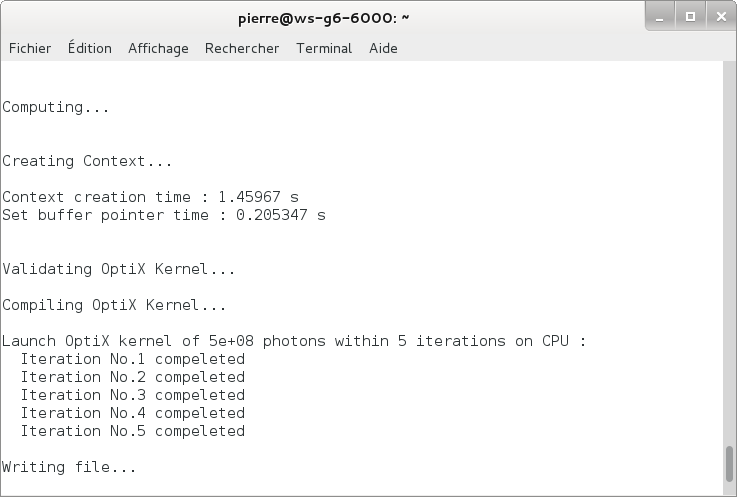
\includegraphics[width=0.7\textwidth]{Figures/500.png}}
\subfigure[1000$\times$1000 kernel]{
\label{sub2}
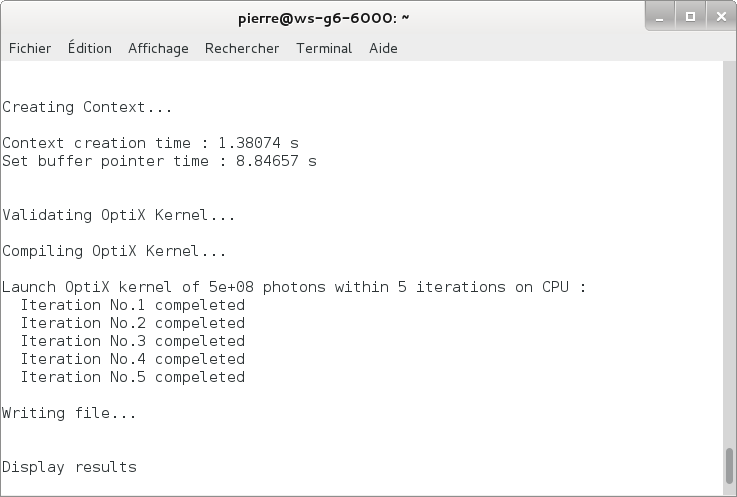
\includegraphics[width=0.7\textwidth]{Figures/1000.png}}
\caption{Initialization difference between 2 kernels.}
\label{fig:kernel}
\end{figure}
The kernel size influences the synchronic computing scale on parallel. Generally speaking, cards with higher Compute Capability could afford larger kernels. But it doesn't mean that a larger kernel is more efficient than a smaller one in any case. With the increment of kernel dimension, latency of block/thread or local/global communication will be extended. For example, two calculations are launched respectively for tracing $5\times10^8$ photons with the same configuration (\fref{fig:kernel}): a first one with a 500$\times$500 kernel and a second one with a 1000$\times$1000 kernel. Though the difference between kernel executions is negligible, we find that the setup of the OptiX device buffer for the 1000$\times$1000 kernel spends almost 44 times longer (8.84 s vs. 0.20 s) than the 500$\times$500 one. There is no formal explanation for the huge variance, but we think this relates to device architecture.
\begin{figure}
\centering
  \subfigure[500$\times$500 kernel for $1\times10^{10}$ photons]{
    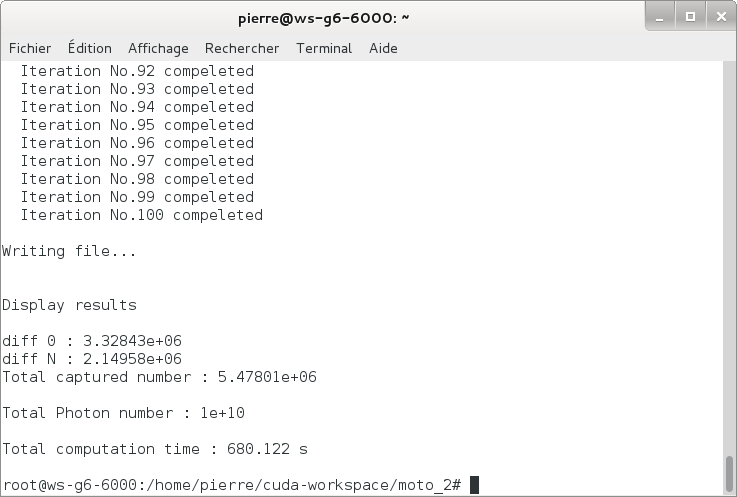
\includegraphics[width=0.7\textwidth]{Figures/500trillion.png}}
  \subfigure[1000$\times$1000 kernel for $1\times10^{10}$ photons]{
    \label{fig:1000}
    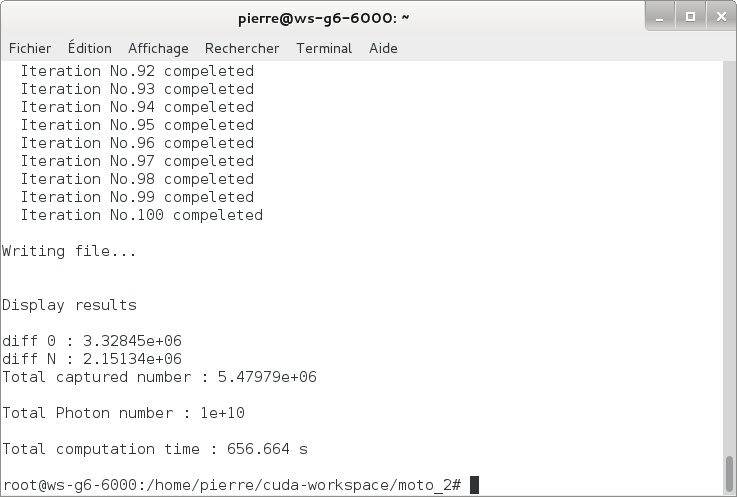
\includegraphics[width=0.7\textwidth]{Figures/1000trillion.png}}
  \caption{Execution time between different kernels.}
  \label{fig:trillion}
\end{figure}

In another test with $1\times10^{10}$ photons, however, we find that even the initialization time is huge. The larger kernel performs more efficiently than the smaller one (\fref{fig:trillion}). This result indicates that a bigger kernel size is more suitable for larger datasets of particle histories. Profiting a maximum kernel dimension and keeping all threads busy will contribute to a better GPU performance.
%----------------------------------------------------------------------------------------

\section{Comparison of Acceleration Structures}
\label{acc}
OptiX encapsulates various acceleration algorithms for ray tracing process. This design liberates users from days of work and knowledges of ray tracing basics. 

Different acceleration structures are evaluated with the same geometry configuration, but it's rather hard to tell the difference. Actually, there are only one sphere and one parallelogram in the test scene and different structures don't vary much in such simple scenes. To be more precise, \textit{NoAccel} (no acceleration) is even better than other structures in our case. This consequence is confirmed by \textit{OptiX Programming Guide} as well: it suggests that for static geometry groups, use \textit{Sbvh} or \textit{TriangleKdTree}. For dynamic geometry groups or large number of elements, experiment with \textit{Lbvh}. For Group nodes , \textit{Bvh} is the best choice in many cases, but if there are few enough children \textit{NoAccel} can be useful \citep{Reference6}.

%----------------------------------------------------------------------------------------

\section{OptiX Performance}
\label{optixperform}
OptiX ray tracing performance is evaluated by comparing it with a CPU cluster. Test configurations are:
\begin{itemize}
  \item \textit{Photon: }number = $1\times10^{10}$, mono-energy = 400 keV, direction = (0,0,-1); 
  \item \textit{Source: }sphere, position = (0,0,0), radius = 1, open angle = $4^{\circ}$;
  \item \textit{Object: }sphere, iron, position = (0,0,-55), radius = 50;
  \item \textit{Detector: }parallelogram, position = (0,0,-110), side length: 10$\times$10, image resolution: 100$\times$100 pixels.
\end{itemize}

The cluster ATHOS uses to link the computing nodes a FDR14 InfiniBand Cable with a bandwidth of 56 Gb/s. It consists of 776 normal nodes and 27 "Bigmem" (up to 2T memory space) nodes. Each normal node contains two Intel Xeon E5-2697 V2 processors (2.7GHz, 12 cores, 30M cache) and a shared memory of 64 GB. 

Firstly, we tested OptiX accuracy by comparing it with the original MODERATO simulation result. One hundred million photons were launched with previous configurations.
\begin{figure}[htbp]
	\centering
		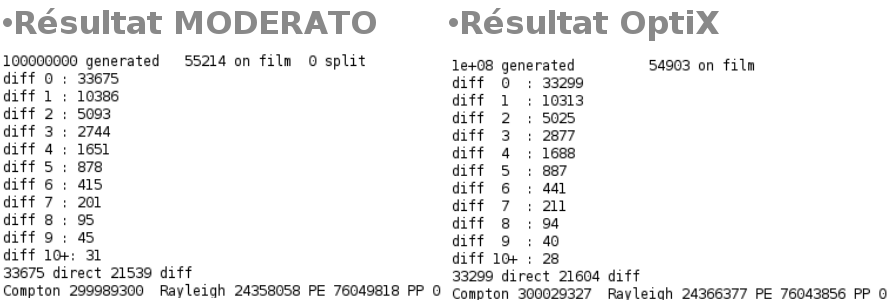
\includegraphics[width=\textwidth]{Figures/test.png}
	\caption{Simulation results of OptiX and MODERATO.}
	\label{fig:test}
\end{figure}

From the above figure, we observe that the difference between these two simulations is reasonable. There is only a small deviation (about $\approx 0.2 \%$) on the final total diffusion number. Moreover, if we reseed the RNG, the result will vary with the same type of deviation. This corresponds well to the Monte Carlo's intrinsic variance since it's based on stochastic processes. This test proves that our implementation works correctly and OptiX can provide enough accuracy for the MODERATO simulation.

\begin{figure}[htbp]
	\centering
		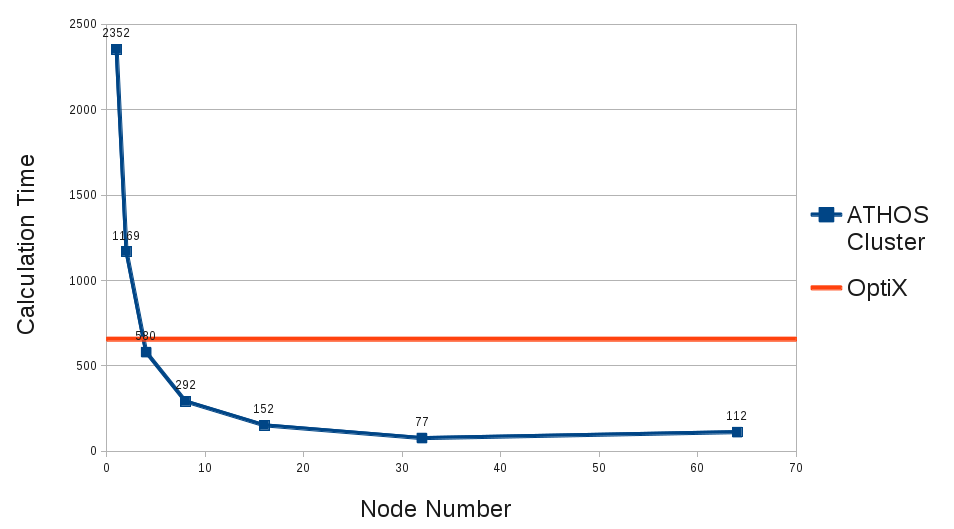
\includegraphics[width=\textwidth]{Figures/cluster.png}
	\caption{Tracing performance with different node amounts on ATHOS cluster.}
	\label{fig:cluster}
\end{figure}

In the second test, calculation time is figured on changing the number of execution nodes on ATHOS. According to \fref{fig:cluster}, we observe that calculation time reduces proportionally with an increment of node numbers. A double nodes brings almost a two-time speedup, but the test with 64 nodes is however longer than that of 32. This decreasing speed-up may come from the increasing data exchange between different nodes, frequent cable latency neutralizes the advantage of large-scale parallelization.

Comparing these results with the OptiX implementation (\fref{fig:1000}), we remark that our OptiX program spend approximately the same time as a 4-node CPU cluster. Note that the GPU we used is just a Quadro (initial for rendering graphics) 2.0 card, such result is rather remarkable and encouraging. Without changing the current code, its performance would be still improved by using a more powerful Tesla card (capability 3.0 or more).

Moreover, eight Xeon E5-2697 processors within the 4-node cluster cost about 20000 dollars. The unit price of Quadro 5000 is only 2499 dollars. In terms of power consumption, a Quadro 5000 consumes ($\approx 150 \ W$) no much more than a single Xeon processor ($\approx 130 \ W$). Those contrasts strongly confirm GPU's giant advantage in terms of performance/price and performance/watt ratios.
%----------------------------------------------------------------------------------------

\section{Technical Assessment}
OptiX's ray tracing potential for general Monte Carlo simulations will be concluded in this section. Advantage and drawbacks will be listed respectively. 
%----------------------------------------------------------------------------------------

\subsection{Advantage of OptiX}
\begin{itemize}
  \item OptiX provides an open ray tracing framework, developers would find it easy to integrate to their own programs. It's also an user-friendly API because programming with OptiX doesn't need too much GPU programming skills. 
  \item It's highly optimized for CUDA architecture so as to get full use of the material, traditional programming difficulties like keeping all threads busy or use of shared memory are automatically managed.
	\item Geometries are totally user-defined, which allows OptiX implementation to preserve the essential analytical description of the original code. Complex geometry with patches is feasible since OptiX supports object-oriented programming on the device.
	\item Built-in simplified mathematical functions reduce calculation time of expensive operations and provide sufficient accuracy for MODERATO. 
  \item Good cost-performance ratio economizes the cost and save energy. More calculations can be operated by cheaper device within shorter time.
\end{itemize}

%----------------------------------------------------------------------------------------

\subsection{Difficulties and Inconveniences}
\begin{itemize}
  \item OptiX manuals are sometimes difficult to understand, users should consult SDK code examples to understand some specific explanations. Few details about OptiX C++ wrapper are included in the programming guide. Several object methods are not even mentioned in the API reference.
  \item Available device cards are confined to NVIDIA's products. Meanwhile, OptiX ray tracing pipeline is not available on the host (no execution on CPU). Thus sustainability of the code is not guaranteed, who knows if NVIDIA still exists after twenty years.
  \item Since the device-side ray tracing pipeline is not object-oriented, several MODERATO models need to be restructured for this mechanism.
  \item Since OptiX 3.5, the API is no longer open-source. Commercial uses are required to pay additional fees, which result in extra cost for selling MODERATO on the market.
  \item Debug of device codes is rather difficult since \textit{printf} is not practical in such large-scale parallel computing.
\end{itemize}

%----------------------------------------------------------------------------------------

\subsection{Following Work}
Future work of our OptiX implementation would take into account the following aspects:
\begin{itemize}
  \item Replace the current XORWOW RNG with MRG32K3A in order to have better statistical characteristics and be more accurate for industrial simulations.
  \item Continue rewriting complex geometry objects on deactivating dynamic allocations. Only the top node of geometry hierarchy can be initialized dynamically on the host. This procedure may take a developer a few weeks.
  \item Implement pair production, electron models in OptiX by using new ray types and creating their own \textit{Materials} bounded to the geometry object. In theory, these modeling processes have no difference with other interaction models and therefore are easy to realize.
  \item Note that material description was highly simplified in the current OptiX implementation: full physic mode, interpolation operations, cross-sections etc, were not full-featured. 
  \item Complete the detector model with OptiX. This part of modeling was not managed during my practice period, so it's hard to estimate the corresponding workload.
\end{itemize}

%----------------------------------------------------------------------------------------